\begin{block}{At a Glance}
  Beginning in Nov. 2015, repeated intense rainfall events associated with mesoscale convective activity caused severe flooding along the Paraguay-Paran\'{a} river system (\cref{fig:study-area}, red box), \emph{displacing over 170000 people}.
  We use a weather typing approch within a diagnostic approach to show that:
  \begin{itemize}
    \item Moisture and energy advection via the South American Low-Level Jet \cite{Marengo:2012cm}, particularly during ``No-Chaco'' events \cite{Vera:2006ib} favored mesoscale convective activity
    \item Strong El Ni\~{n}o favored strong SALLJ but MJO and Atlantic dipole pattern contributed to jet exit region (thus No-Chaco SALLJ events)
    \item Raw S2S model forecasts of rainfall had limited skill beyond 10-15 days, but statistical methods -- particularly the PCR and CCA methods that correct both spatial patterns and magnitudes -- substantially improve forecast skill
  \end{itemize}
  \begin{mdframed}
  \begin{figure}
  	\noindent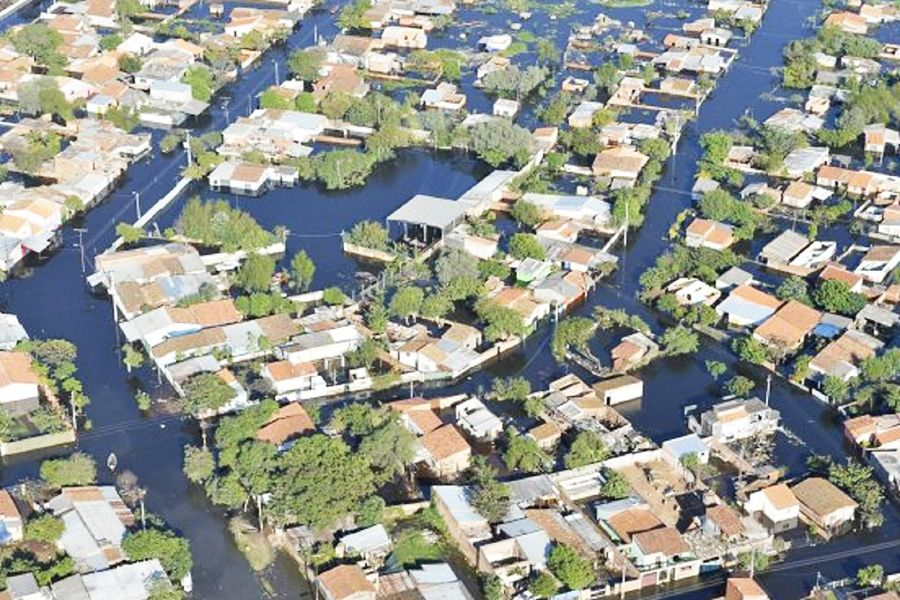
\includegraphics[width=0.45\textwidth]{asuncion-inundaciones.jpg}~
    \noindent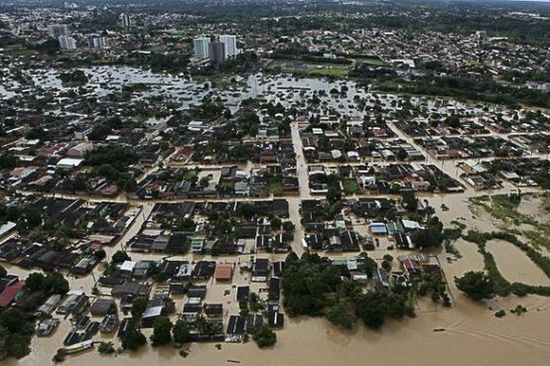
\includegraphics[width=0.45\textwidth]{rio-py-banados.jpg}
  	\caption{
  		Asuncion, Paraguay, 2015-16
  	}
    \label{fig:floods}
  \end{figure}
  \end{mdframed}
\end{block}
